\documentclass[letterpaper,12pt]{article}
\usepackage{graphicx}
\usepackage{listings}
\usepackage[super]{nth}
\usepackage[hyphens]{url}
\usepackage{hyperref}
\usepackage{amsmath}
\usepackage[makeroom]{cancel}
\usepackage[table]{xcolor}
\usepackage{comment}
\usepackage[space]{grffile}


\newcommand*{\srcPath}{../src}%

\lstset{
	basicstyle=\footnotesize,
	breaklines=true,
}

\begin{document}

\begin{titlepage}

\begin{center}

\Huge{Assignment 1}

\Large{CS 532:  Introduction to Web Science}

\Large{Spring 2018}

\Large{Hrishikesh Gadkari}

\Large Finished on \today

\end{center}

\end{titlepage}

\newpage


% =================================
% First question
% =================================
\section*{1}


\subsection*{Question}

\begin{verbatim}
1.  Demonstrate that you know how to use "curl" well enough to
correctly POST data to a form.  Show that the HTML response that
is returned is "correct".  That is, the server should take the
arguments you POSTed and build a response accordingly.  Save the
HTML response to a file and then view that file in a browser and
take a screen shot.
\end{verbatim}

\subsection*{Answer}

To Post data to a form using curl I used the following command:

\lstinputlisting[frame=single,caption={Curl command to post data},label=lst:q1fetch,captionpos=b,numbers=left,showspaces=false,showstringspaces=false,basicstyle=\footnotesize]{curl.sh}

To approach this problem I referred the \url{https://gist.github.com/subfuzion/08c5d85437d5d4f00e58} url.

The use of each of the command options mentioned in Listing 1 is as follows:

\begin{itemize}
  \item -i: To include HTTP headers in the response
  \item -d: Send specified data in POST request which is followed by the data(parameters) to be sent to the form
  \item -X: The request method to be used. In this case we have used POST method followed by the php page where data is to be posted
\end{itemize}

The output in the terminal looks as displayed below:

\clearpage

\begin{figure}[h]
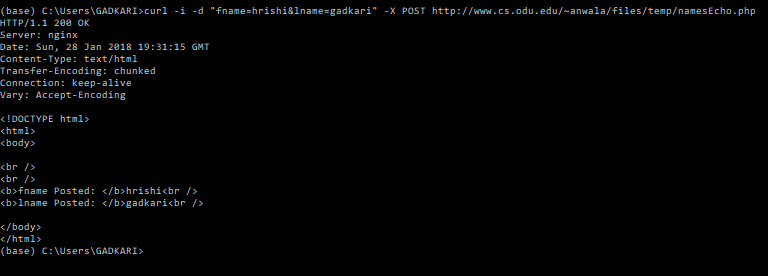
\includegraphics[scale=0.8]{Response.png}
\caption{ Response rendered in terminal}
\label{fig:q1Response}
\end{figure}



The image below displays the view of the output in the browser after saving it in output.html file.

\begin{figure}[h]
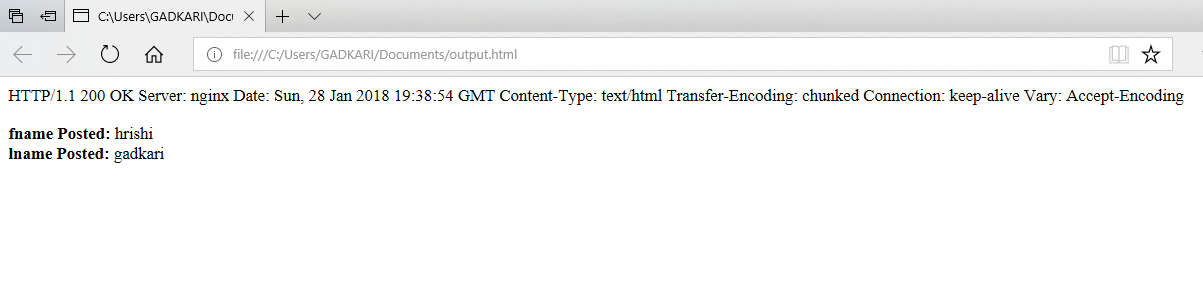
\includegraphics[scale=0.5]{WebResponse.png}
\caption{Response rendered in browser}
\label{fig:q1BrowserResponse}
\end{figure}


\clearpage

% =================================
% Second question
% =================================

\section*{2}

\subsection*{Question}

\begin{verbatim}
2.  Write a Python program that:
  1. takes as a command line argument a web page
  2. extracts all the links from the page
  3. lists all the links that result in PDF files, and prints out
     the bytes for each of the links.  (note: be sure to follow
     all the redirects until the link terminates with a "200 OK".)
  4. show that the program works on 3 different URIs, one of which
     needs to be: 
     http://www.cs.odu.edu/~mln/teaching/cs532-s17/test/pdfs.html
\end{verbatim}

\subsection*{Answer}

To solve the above problem I wrote the following script using Python3:

\lstinputlisting[frame=single,caption={Python script that searches for links that end in pdf files},label=lst:q2fetch,captionpos=b,numbers=left,showspaces=false,showstringspaces=false,basicstyle=\footnotesize]{crawl.py}


The following libraries were used in my script:

\begin{itemize}
  \item Beautiful Soup: To parse the HTML and XML documents and extract the data(third party library)
  \item sys: This module provides access to some variables used or maintained by the interpreter and to functions that interact strongly with the interpreter
  \item requests: To make HTTP requests
  \item urllib: This package collects several modules for working with URLs
  \item urlparse: Focuses on splitting a URL string into its components, or on combining URL components into a URL string
  \item urljoin: To append a url to the base url
\end{itemize}

My solution took an iterative approach doing one URI at a time and waiting for each response until moving onto the next URI found.

For the part 1 of the problem the program first checks whether the number of arguments are correct using the command line arguments and if correct, it will pass the first argument after the script name  and considers only a properly formatted URI and performs a HTTP get request using the requests library. To check whether the URI is redirected to a new address, response.history \cite{historyref} was used, after which get request is made to the new URI.

For the part 2 of the problem, that is to extract all links (absolute as well as relative) from the website, Beautiful Soup \cite{beautifulsoupref} as a third party library was used to find all the html a elements that contained href tags using the specified lxml parser.

For the part 3 of the problem, the program iterates through each of the URIs found on the page and request again each of those URIs to determine if the URI would point to pdf file.  Also if the program encounters a relative link it appends the base url with the relative url. The flow behind this is that it first checks whether the link is absolute using urlparse(web).netloc \cite{urllibref}. If False it changes the link into absolute link using urljoin() \cite{parseref}. For this I referred stackoverflow website \cite{urlref}. After this using head and get requests, the content-type, content-length and status code are obtained for each of the URIs and checks whether it returns status-code \cite{urllibref} as 200 or if the URI has redirects \cite{historyref} and also if content-type \cite{urllibref} is PDF, thus giving the PDF link for the Final URI.

The script is ran with the command as shown below: 

\begin{lstlisting}[frame=single]
python crawl.py URI
\end{lstlisting}

The URIs I used for this problem were:

\begin{itemize}
  \item \url{http://www.cs.odu.edu/~mln/teaching/cs532-s17/test/pdfs.html}
  \item \url{http://www.cs.odu.edu/~mweigle/}
  \item \url{http://www.cs.odu.edu/~yaohang/}(the output displays a relative link which is converted to absolute and eventually giving a pdf link)
\end{itemize}

The output for each of the URIs is displayed below:

\lstinputlisting[frame=single,caption={Output from \url{http://www.cs.odu.edu/~mln/teaching/cs532-s17/test/pdfs.html}},label=lst:q2URI1,captionpos=b,numbers=left,showspaces=false,showstringspaces=false,basicstyle=\footnotesize]{uri1.txt}

\lstinputlisting[frame=single,caption={Output from \url{http://www.cs.odu.edu/~mweigle/}},label=lst:q2URI2,captionpos=b,numbers=left,showspaces=false,showstringspaces=false,basicstyle=\footnotesize]{uri2.txt}

\lstinputlisting[frame=single,caption={Output from \url{http://www.cs.odu.edu/~yaohang/}},label=lst:q2URI3,captionpos=b,numbers=left,showspaces=false,showstringspaces=false,basicstyle=\footnotesize]{uri3.txt}


\clearpage

% =================================
% Third question
% =================================

\section*{3}

\subsection*{Question}

\begin{verbatim}
3.  Consider the "bow-tie" graph in the Broder et al. paper (fig 9):
    http://www9.org/w9cdrom/160/160.html

    Now consider the following graph:

    A --> B
    B --> C
    C --> D
    C --> A
    C --> G
    E --> F
    G --> C
    G --> H
    I --> H
    I --> K
    L --> D
    M --> A
    M --> N
    N --> D
    O --> A
    P --> G 
    
    For the above graph, give the values for:

    IN: 
    SCC: 
    OUT: 
    Tendrils: 
    Tubes: 
    Disconnected:
\end{verbatim}

\clearpage
\subsection*{Answer}

A graph was generated for the above values using webgraphviz \cite{webgraphvizref}. The following snippets show how it got generated:

\begin{figure}[h]
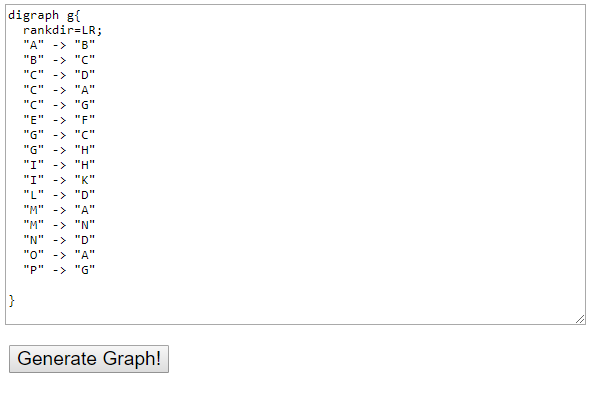
\includegraphics[scale=0.7]{graph1.png}
\caption{Graph generation with WebGraphviz}
\label{fig:q3graph1}
\end{figure}

\begin{figure}[h]
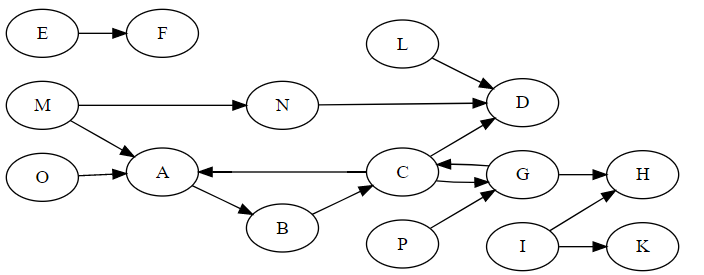
\includegraphics[scale=0.6]{graph2.png}
\caption{Graph generated with WebGraphviz}
\label{fig:q3graph2}
\end{figure}

As per the figure 9 in Broder et al. paper and also from the reference to \url{https://www.harding.edu/fmccown/classes/comp475-s13/web-structure-homework.pdf}, it made my approach clear to this problem that I should start from SCC. From my observation the values could be as follows:

\textbf{SCC:} A, B, C, G

Since SCC is at the center of the graph, it will contain values which have directed links amongst each other and also have in-links or out-links to other nodes outside of SCC. 

\textbf{IN:} M, O, P

Values which have no in-links but can reach the SCC values are considered as IN values.

\textbf{OUT:} D, H

Values which have in-links from SCC values but have no out-links are considered as OUT values.

\textbf{Tendrils:} I, K, L

Values which have out-links to OUT values and have in-links from IN values but do not refer to SCC values at any point are considered as Tendrils. 

\textbf{Tubes:} N

Value which is in the middle of IN and OUT value and acts as a direct path from IN to OUT but do not refer to SCC at any point is considered as a Tube.

\textbf{Disconnected:} E, F

These values do not connect to anything in the graph, but only amongst them.

\clearpage


\clearpage

% =================================
% Bibliography
% =================================

\begin{thebibliography}{9}
\bibitem{urllibref} 
"Urllib.requests Documentation." Developer Interface — Requests 2.18.4 documentation, Web. 28 Jan, 2018. \url{https://docs.python.org/3.0/library/urllib.request.html}. 
\bibitem{beautifulsoupref} 
Richardson, Leonard. "Beautiful Soup Documentation." Beautiful Soup Documentation - Beautiful Soup 4.4.0 Documentation. N.p., n.d. Web. 28 Jan. 2018. \url{https://www.crummy.com/software/BeautifulSoup/bs4/doc/}.
\bibitem{parseref} 
"Urllib.parse Documentation." 21.8. urllib.parse — Parse URLs into components — Python 3.6.4 documentation, Web. 28 Jan. 2018. \url{https://docs.python.org/3/library/urllib.parse.html}.
\bibitem{historyref} 
Martijn Pieters. "How to Check Redirects using Python?" Stack Overflow. N.p., n.d. Web. 28 Jan. 2018. \url{https://stackoverflow.com/questions/20475552/python-requests-library-redirect-new-url}.
\bibitem{urlref} 
Lalinský, Luká¨. "How Can I Check If a URL Is Absolute Using Python?" Stack Overflow. N.p., n.d. Web. 28 Jan. 2018. \url{https://stackoverflow.com/questions/8357098/how-can-i-check-if-a-url-is-absolute-using-python}.
\bibitem{webgraphvizref} 
"Webgraphviz." Webgraphviz. N.p., n.d. Web. 28 Jan. 2018. \url{http://www.webgraphviz.com/}.
\end{thebibliography}

\end{document}